\label{chap:implementation}
%FIXME: V1 decoder logic
%FIXME: original SCB
%FIXME: Add information about the development history thingies from the repo
%FIXME: my research group's arrays?
%FIXME: talk about fw control modularity
This chapter describes an FPGA implementation of the PDP architecture\cite{LandwehrEtAl2019_2,JacksonEtAl2019,BrowningEtAl2020}. For the purposes of this discussion, only relevant details are included to ease the readers understanding. First, the chapter will discuss the purpose of the implemented architecture. Following this each component will be discussed at a high-level. Finally, the operation of sub-components will be discussed.
\section{HDMI Transport Layer}
    \label{sec:hdmi_transport_layer}
    %FIXME: Discuss goal 4
    \begin{figure}
        \centering
        
\includegraphics[width=0.5\textwidth]{fig/packet_refresher.pdf}
        \caption{Packet Format Refresher}
        \label{fig:packet_refresher}
    \end{figure}
    \begin{figure}
        \centering
        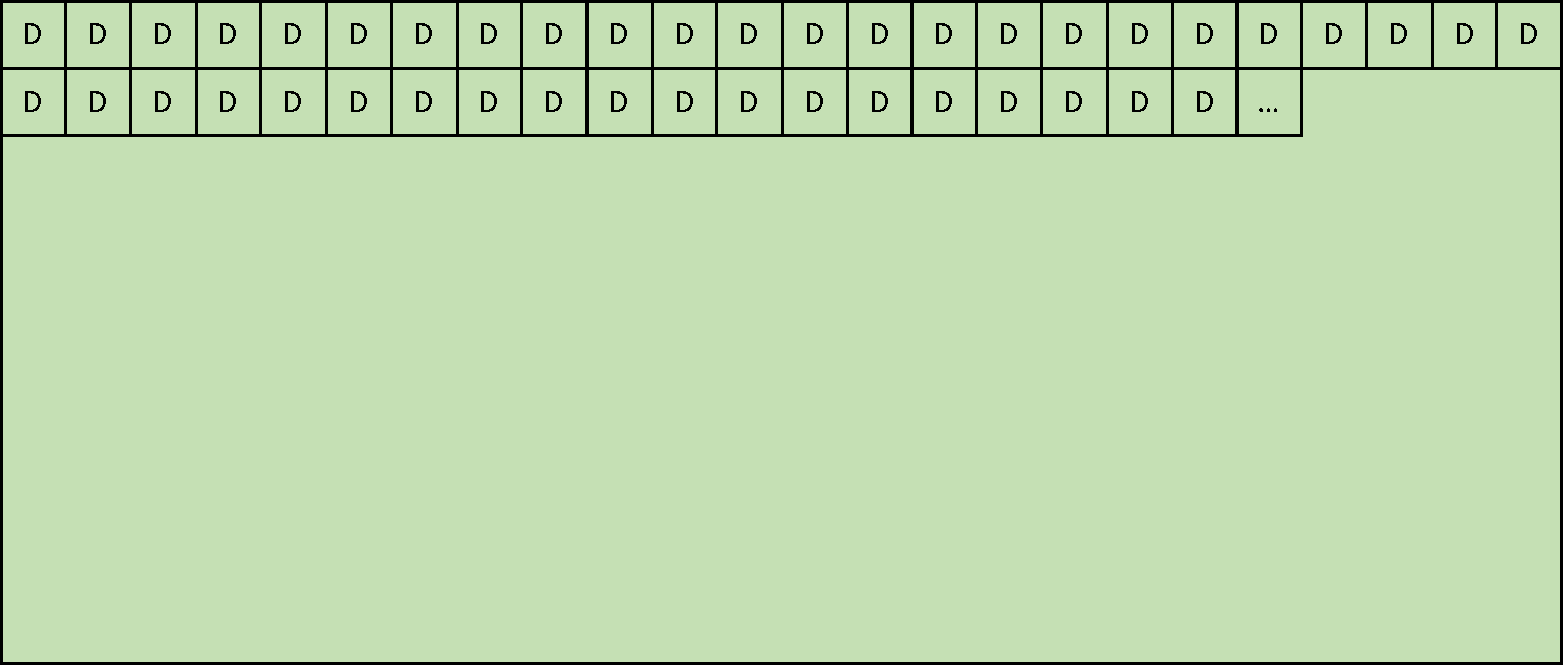
\includegraphics[width=1.0\textwidth]{fig/classic_video.pdf}
        \caption{Normal Frame with Display Data}
        \label{fig:classic_video}
    \end{figure}
    \begin{figure}
        \centering
        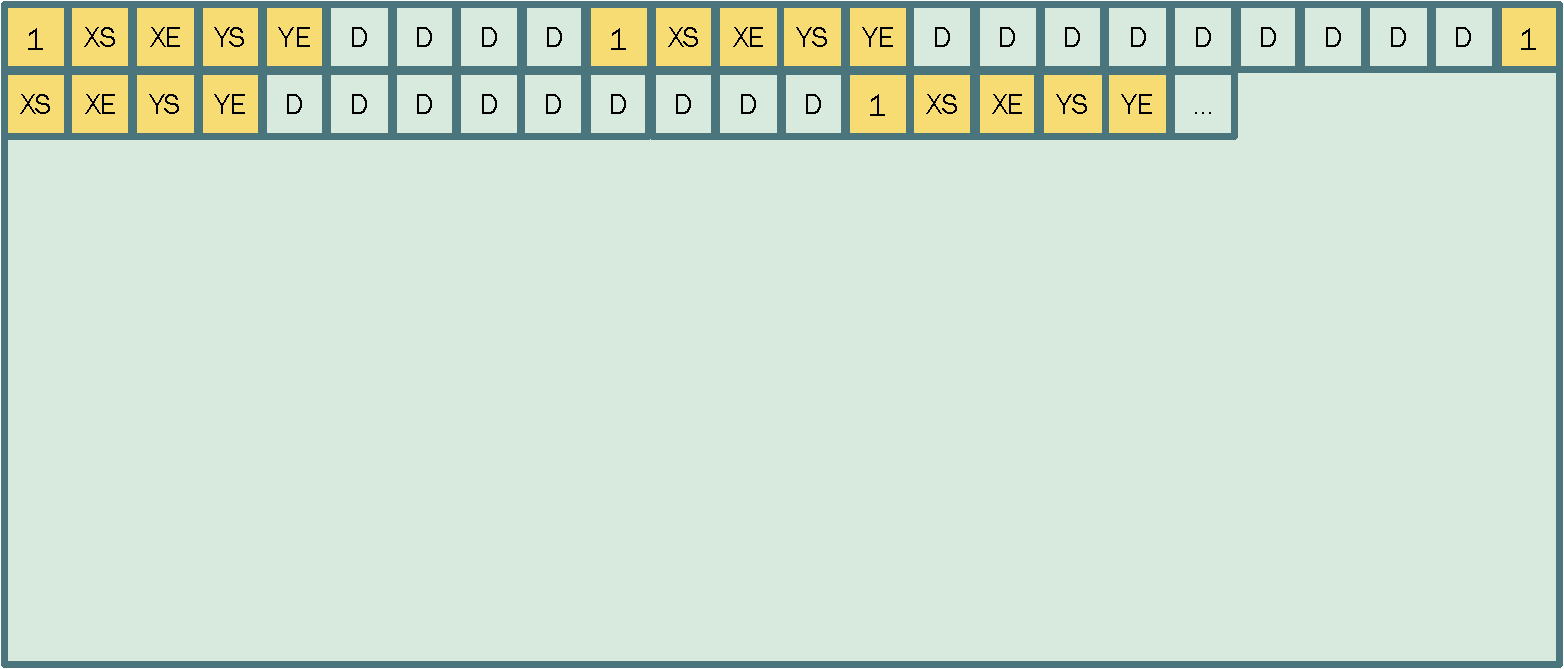
\includegraphics[width=1.0\textwidth]{fig/embedded_frame.pdf}
        \caption{Embedded PDP Frame}
        \label{fig:embedded_frame}
    \end{figure}
    \begin{figure}
        \centering
        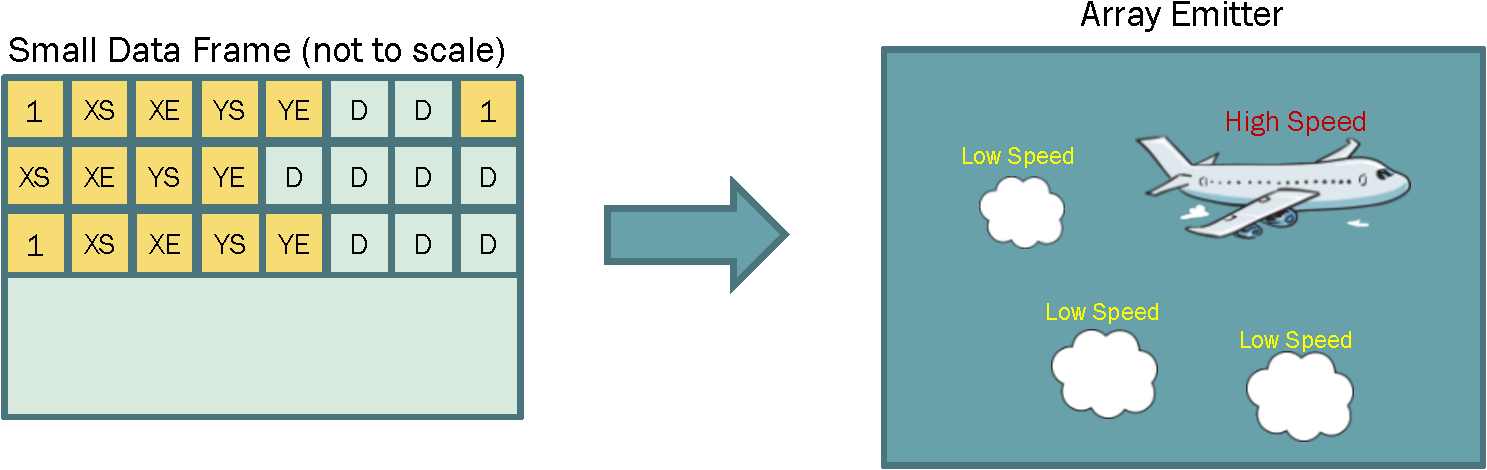
\includegraphics[width=1.0\textwidth]{fig/embedded_frame_to_emitter.pdf}
        \caption{Embedded PDP Frame to Array Mapping}
        \label{fig:embedded_frame_to_emitter}
    \end{figure}

\section{Abstract Architecture}
    \begin{figure}
        \centering
        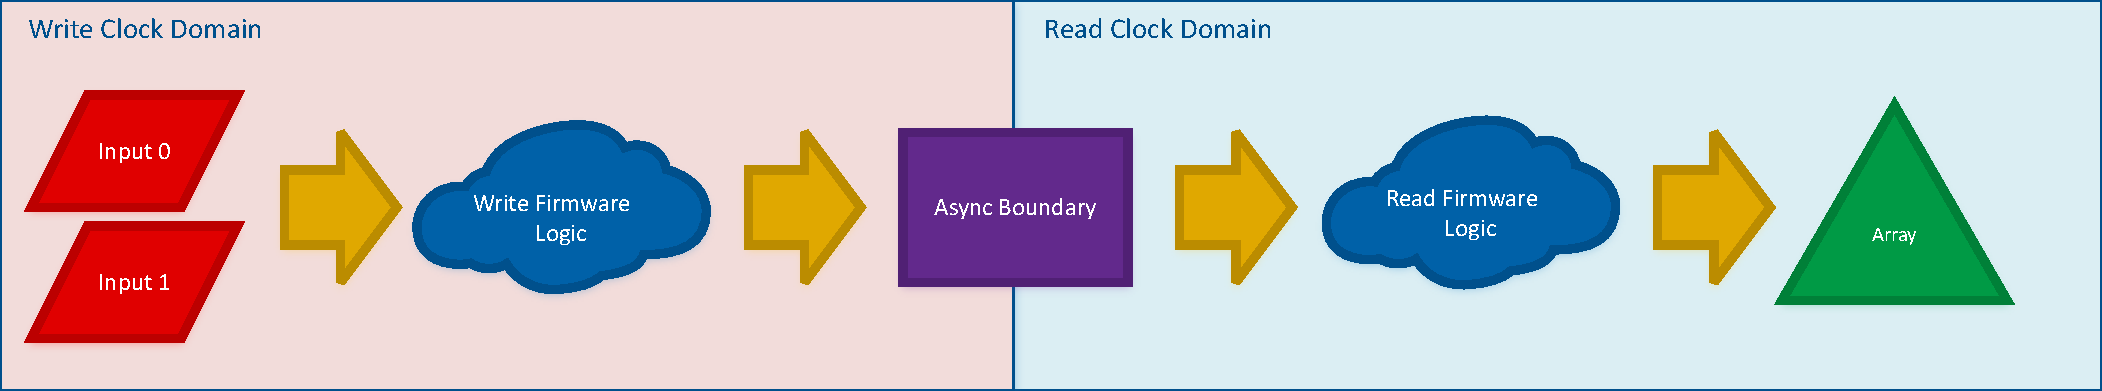
\includegraphics[width=1.0\textwidth]{fig/abstract_architecture.pdf}
        \caption{Abstract PDP Firmware Architecture}
        \label{fig:abstract_architecture}
    \end{figure}

\section{Frontend Architecture}
    \label{sec:frontend_arch}

\section{Overall Backend Architecture}
    \label{sec:backend_arch}
    The implemented architecture consists of the portion of the AMM that drives an IRLED tile (or emitter array) directly from data packets sent by a compositor. As such, it is responsible for receiving PDP packets, decoding, validating, and drawing them to an IRLED array. This is shown in Figure~\ref{fig:overall_arch}. In the current implementation, packets are sent using an underlying HDMI protocol layer. The incoming data is synchronized across two distinct clock domains utilizing a synchronized circular buffer (SCB). The input side consists of two separate HDMI inputs in order to meet system bandwidth requirements. Each input is assumed to contain clock skew relative to the other so separate SCBs are used to synchronize these to the system domain. At a high-level, individual data words of 24-bit sized values come in per HDMI cycle. These are transitioned to the system domain and stored for retrieval by the array emitter module. The array emitter module is responsible for bringing in each 24-bit word value and emptying the corresponding SCB slot. As it brings in each word, it begins to decode them into PDP commands. Once enough data is buffered for a write or reset command, it sends the data to the write buffer module which then drives an emitter directly through I/O lines.

    \begin{figure}
        \centering
        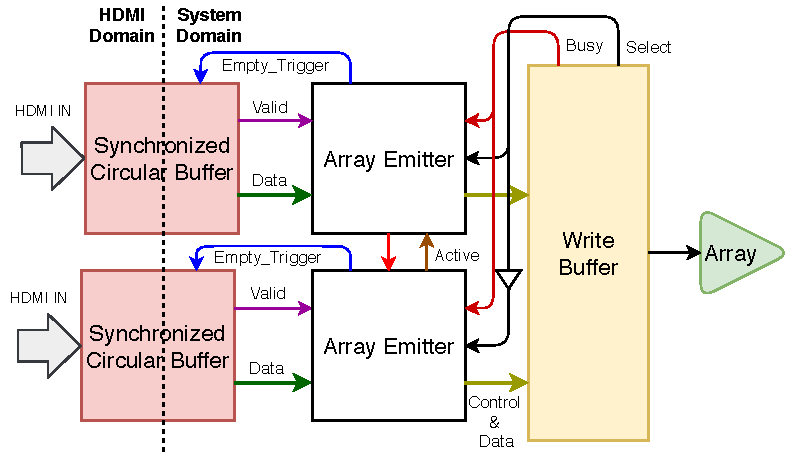
\includegraphics[width=1.0\textwidth]{fig/pdp_overall_arch.pdf}
        \caption{Overall PDP Backend Architecture}
        \label{fig:overall_arch}
    \end{figure}

\section{Synchronized Circular Buffer}

    Figure~\ref{fig:scb_arch} shows the submodule details of the synchronized circular buffer utilized in the implementation. Internally, it consists of two controllers, two data routers, and the actual internal buffer storage with a built-in synchronizer circuit, and a write buffer connected to I/O pins.

    \begin{figure}
        \centering
        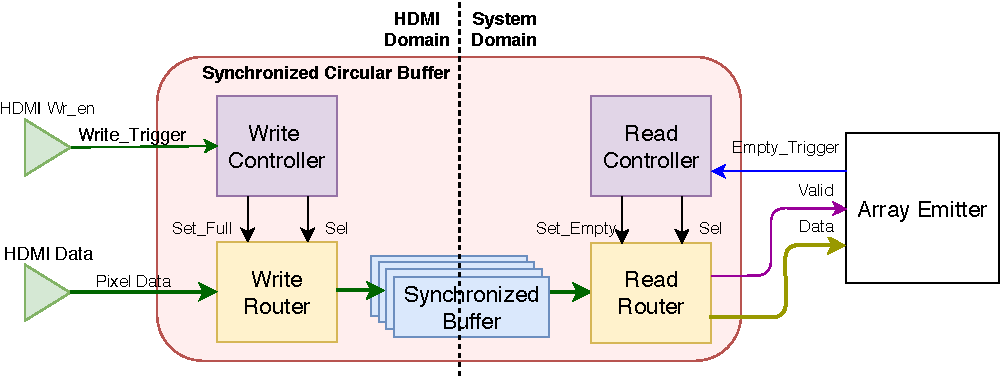
\includegraphics[width=1.0\textwidth]{fig/pdp_scb_arch.pdf}
        \caption{Synchronized Circular Buffer Architecture}
        \label{fig:scb_arch}
    \end{figure}

    The write controller is used to coordinate which internal buffer to write data to. A buffer is marked as full when a trigger comes in, and a new buffer is selected when the previous is filled. This is triggered via an external write enable signal sent from HDMI. The write router does the actual data redirection based off the buffer selected by the write controller. At high-level, internally, a request-acknowledgment handshake is used to ensure the data has transitioned correctly across clock domains and is available on the other side. The details of this implementation will be discussed in Chapter~\ref{Sec:MemorySync}. Once data becomes available, the read router will output the data linesas well as a valid signal indicating that the data can be read and cleared. The read controller will clear it once an empty trigger is sent from the array emitter indicating that the corresponding word has been read. It will then select the next buffer. Once the last buffer is written or read by either controller, the first buffer will be selected again. To note here for clarity, the actual filling and clearing of the buffers is done by HDMI write enable on the writer side, and the array emitter on the reader side.

    \subsection{Controllers}

    \subsection{Routing}

    \subsection{Internal Buffer and Memory Synchronizer}
    \label{Sec:MemorySync}

    Figure~\ref{fig:sb_arch} shows the internals of the internal buffers used by the SCB.
    \begin{figure}
        \centering
        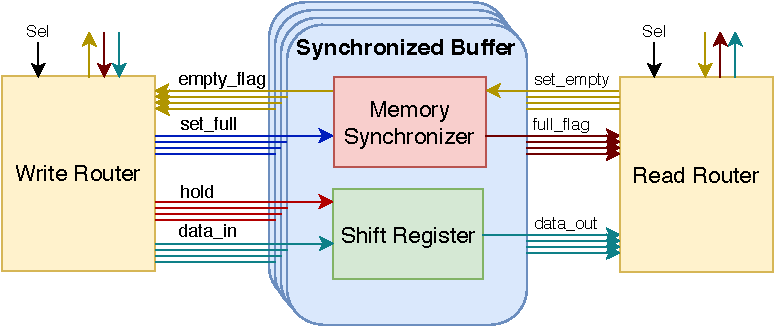
\includegraphics[width=1.0\textwidth]{fig/pdp_sb_arch.pdf}
        \caption{Synchronized Internal Buffer Architecture}
        \label{fig:sb_arch}
    \end{figure}

    Figure~\ref{blah} shows the internals of the memory synchronizer utilized by the SCB architecture.

\section{Array Emitter}

    Figure~\ref{fig:ae_arch} shows the details of the array emitter module used in the implementation. Internally, the array emitter consists of individual controllers that each perform a particular role. Currently these are the write enable controller, which controls writing draw region packets; the reset controller, which controls the resetting process per frame; and the valid controller which does validation checks on the input in order to verify the correctness of packets. Each controller takes in similar input signals and produces similar output signals with some exceptions depending on the actual function of the individual controller module. On the input side, each controller takes in a valid and data line corresponding to an individual word of a PDP packet. Additionally, an active line is brought into each controller to indicate whether another controller module is active or not. This is used to ensure that other modules do not become active (for correctness purposes) while another is currently processing a packet. During an idle phase, the write enable and reset controllers will wait for a corresponding packet ID to come in.

    \begin{figure}
        \centering
        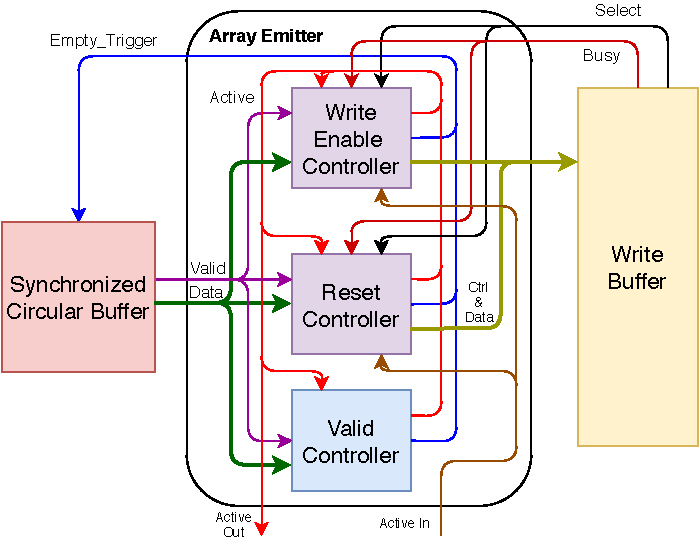
\includegraphics[width=1.0\textwidth]{fig/pdp_ae_arch.pdf}
        \caption{Array Emitter Architecture}
        \label{fig:ae_arch}
    \end{figure}


\section{Write Buffer}
     Figure~\ref{fig:wb_arch} shows the details of the write buffer architectures inputs and outputs along with important signaling to other modules. The write buffer is responsible for driving the I/O pins that go to the array.

    \begin{figure}
        \centering
        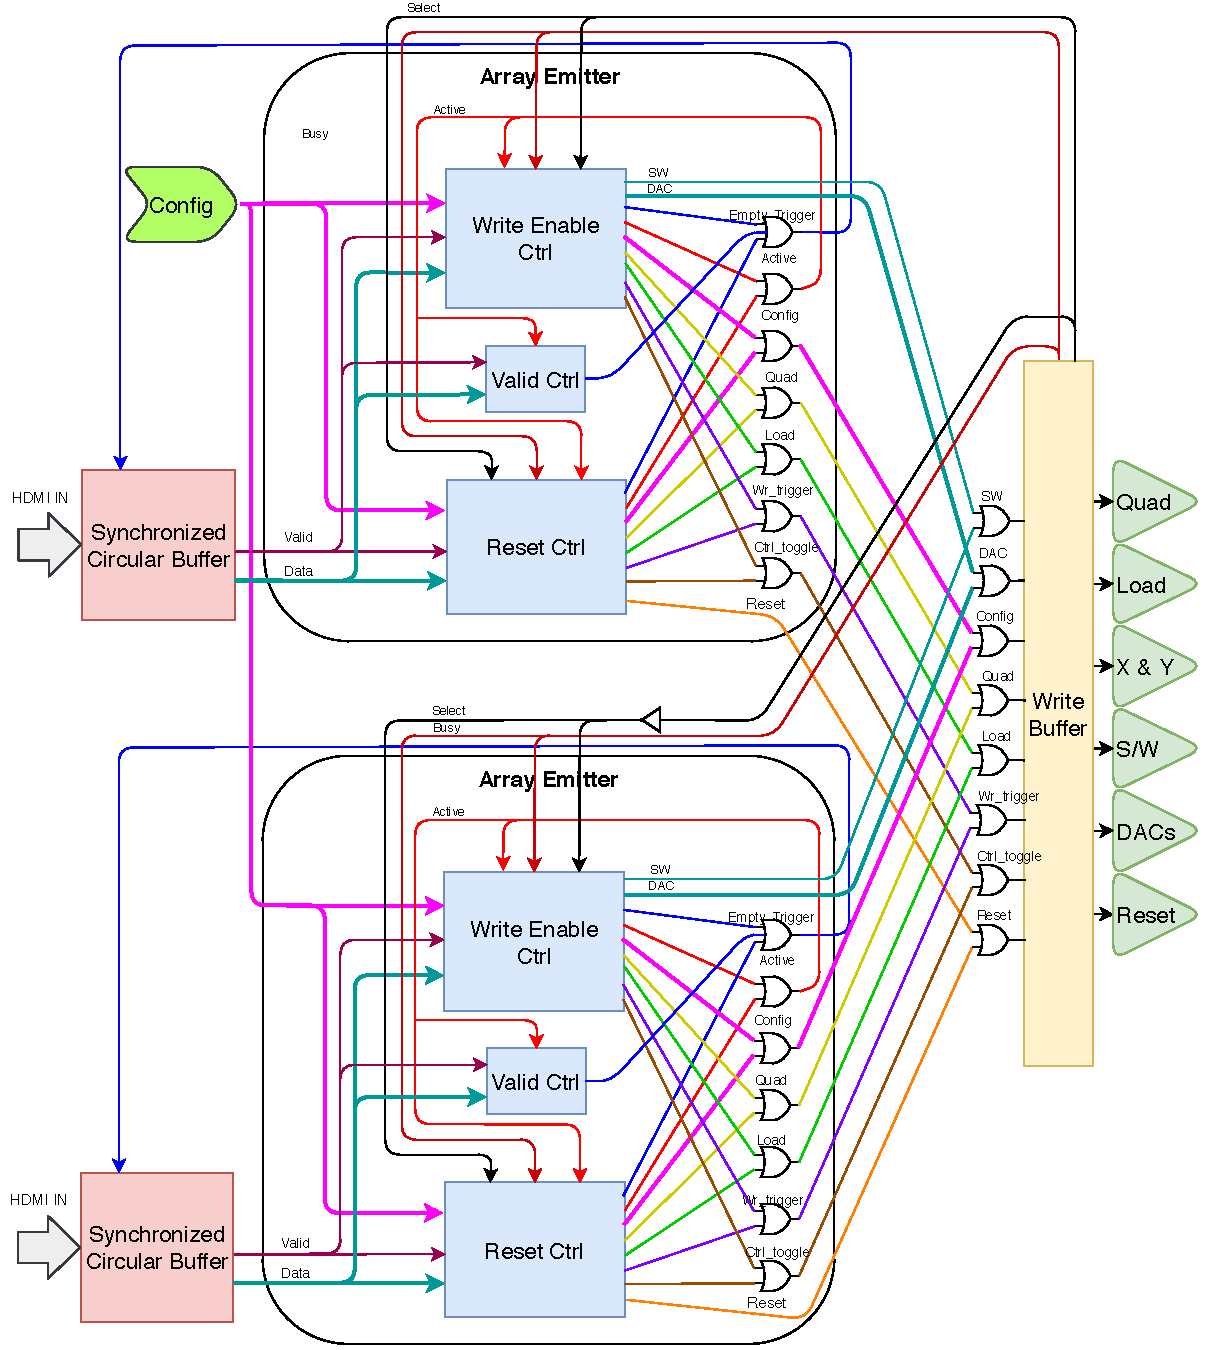
\includegraphics[width=1.0\textwidth]{fig/pdp_wb_arch.pdf}
        \caption{Write Buffer Architecture}
        \label{fig:wb_arch}
    \end{figure}

\section{State Machine}
    When a packet ID matching an operation handled by a given controller arrives, the corresponding controller will switch states and then wait for the rest of the incoming packet data to arrive. This is shown in Figure~\ref{fig:state_machine}. For example, item 3 shows each state machine waiting for a corresponding PDP OP code. If a draw region packet ID were to arrive, then the state machine would wait for the X start address, X end address, Y start address, and Y end address shown in item 4. Finally, the state machine would buffer the needed data for a write and move to the write state once all data has been buffered. In the write state it would send the data to the write buffer. If more data needed to be written for the PDP packet, it would then continue buffering the needed data, and wait for the write buffer to be idle to send the next set of data. The busy line in Figure~\ref{fig:ae_arch} indicates when the write buffer is in the process of writing to the array. This would continue until all data was written for the packet, finally proceeding to the idle state. The reset controller contains similar logic, but for the reset process. The valid controller is used to ensure that incorrect or corrupt packet data is cleared. If an invalid packet OP code arrives during an array emitter idle phase, the valid controller will simply empty the corresponding SCB slot. In future revisions, it will perform CRC checks on packet data to ensure the header and body are valid. The Active-Out, Active-In, and Select lines are used to coordinate which array emitter module has control over the write buffer. After an array write, normally an array emitter will signal the write buffer that it is ceding control to the other array emitter, but only in cases where the other array emitter is currently active and waiting to write.

    \begin{figure}
        \centering
        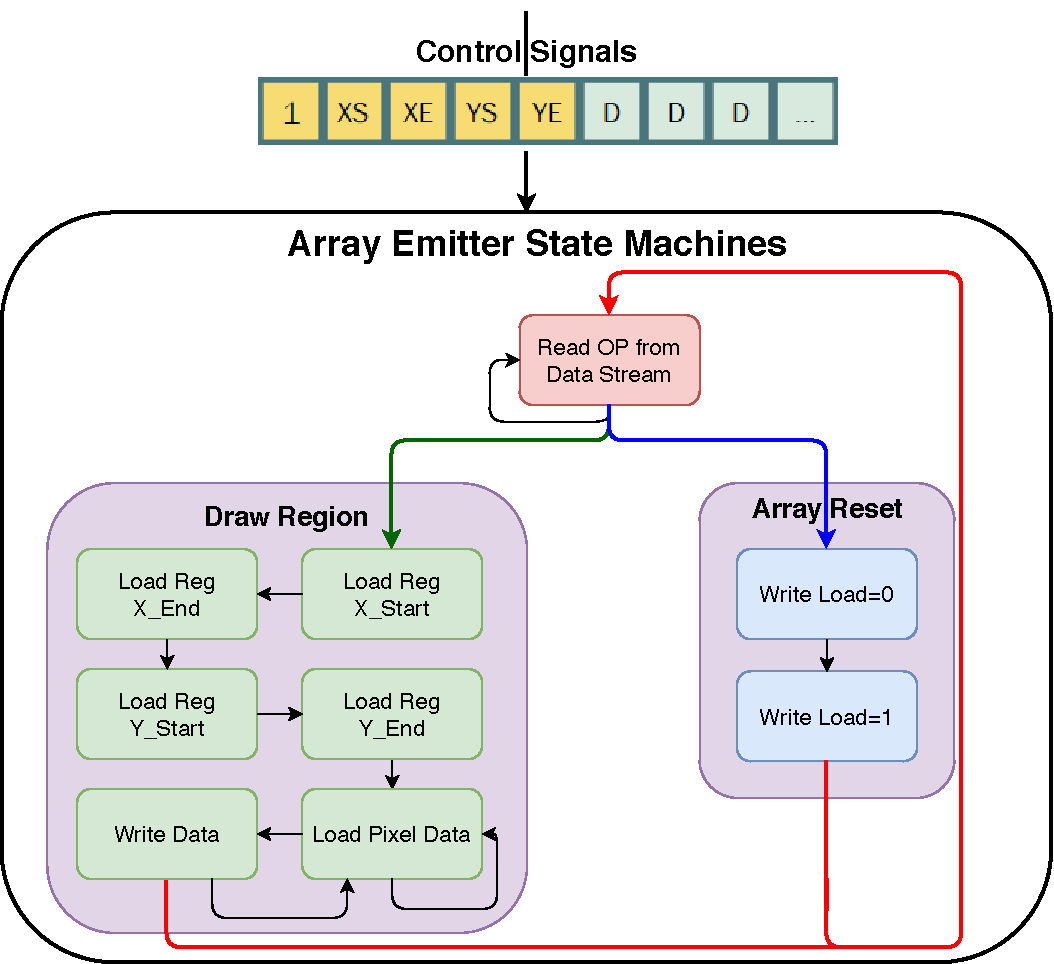
\includegraphics[width=1.0\textwidth]{fig/pdp_state_machine.pdf}
        \caption{PDP State Machine}
        \label{fig:state_machine}
    \end{figure}
